\documentclass[a4paper,10pt]{beamer}
\usetheme{}
\usepackage[french]{babel}
\usepackage[T1]{fontenc}
%\usetheme{Boadilla}
%\usetheme{AnnArbor}
\usecolortheme{crane}
\setbeamertemplate{navigation symbols}{}
\setbeamertemplate{footline}[frame number]
\usefonttheme{serif}
\usepackage[applemac]{inputenc}
\usepackage{lmodern}
\usepackage{microtype}
\usepackage{hyperref}
\usepackage{dsfont}
\usepackage{amsmath}
\usepackage{mathenv}
\usepackage{amsthm}
\usepackage{graphicx}
\newcommand{\e}{\mathrm{e}}
\newcommand{\w}{\omega}
\newcommand{\dd}{\mathrm{d}}
\newcommand{\id}{\mathrm{id}}
\newcommand{\Id}{\mathrm{Id}}
%\newcommand{\x}{\times}
%\renewcommand{\x}{\mathbf{x}}
\newcommand{\Z}{\mathbb{Z}}
\newcommand{\Q}{\mathbb{Q}}
\newcommand{\R}{\mathbb{R}}
\newcommand{\C}{\mathbb{C}}
\newcommand{\N}{\mathbb{N}}
\newcommand{\T}{\mathbb{T}}
\newcommand{\Acal}{\mathcal{A}}
\newcommand{\Ccal}{\mathcal{C}}
\newcommand{\Pcal}{\mathcal{P}}
\newcommand{\Fcal}{\mathcal{F}}
\newcommand{\Scal}{\mathcal{S}}
\newcommand{\ra}{\rightarrow}
\renewcommand{\P}{\mathbf{P}}
\newcommand{\pau}{}
\newcommand{\Repac}{\mathrm{Rep}_{\mathrm{ac}}}


\newtheorem{lemme}[theorem]{Lemme}
\newtheorem{thm}[theorem]{Th\'eor\`eme}

\theoremstyle{plain}
\newenvironment{remark}



%\AtBeginSection[]{
  %\begin{frame}{Summary}
  %\small \tableofcontents[currentsection, hideothersubsections]
  %\end{frame} 
%}

\title{\textbf{Syst\`emes dynamiques}}
\subtitle{TD n�8}
\date{10 novembre 2020}
\author[Yann Chaubet]{Yann Chaubet}
%\institute[Universit\'e Paris-Sud]{\inst{1} Universit\'e Paris-Sud}

\begin{document}


\begin{frame}
\maketitle
\end{frame}

\begin{frame}{Exercice 1}
\textbf{1}. On consid\`ere une fonction $f$ d\'efinie au voisinage de $0 \in \R^n$ telle que $\dd f_0 = 0$, et $\varphi = (\varphi^1, \dots, \varphi^n)$  un diff\'eomorphisme local au voisinage de $0$, tel que $\varphi(0) = 0$.

 %\pau
\vspace{0.2cm}

On calcule
$$
\begin{aligned}
\partial_k \partial_\ell (f\circ \varphi) &= \sum_{i} \partial_k\left([(\partial_i f) \circ \varphi] \partial_\ell \varphi^i \right) \\
&= \sum_{i} [(\partial_if) \circ \varphi] \partial _k \partial_\ell \varphi^i + \sum_{j,i} [(\partial_i \partial_j f) \circ \varphi] (\partial_k \varphi^i)(\partial_\ell \varphi^j).
\end{aligned}
$$

 %\pau
\vspace{0.2cm}

Puisque $\dd f_0 = 0$ on obtient
$$
\mathrm{Hess}_{f\circ \varphi}(0) = (\dd \varphi_0)^{\top} \mathrm{Hess}_f(0) (\dd \varphi_0),
$$
ce qui conclut.

\end{frame}

\begin{frame}

\textbf{2.} On remarque qu'une fonction de Morse a un nombre fini de points critiques, car ils sont isol\'es. 

 %\pau
\vspace{0.2cm}

De plus la condition "$\mathrm{Hess}_f(0)$ est non d\'eg\'en\'er\'ee" est ouverte, ce qui conclut.

 %\pau
\vspace{0.2cm}

\textbf{3.} On suppose $\varphi_{\tau}(x) = x$ avec $\tau > 0$. Calculons 
$$
\begin{aligned}
\partial_t f(\varphi_t(x)) &= \dd f_{\varphi_t(x)}(X(\varphi_t(x)))�\\
&= - \dd f_{\varphi_t(x)}(\nabla^g f(\varphi_t(x)))  \\
&= -g_{\varphi_t(x)}(\nabla^g f(\varphi_t(x)), \nabla^g f(\varphi_t(x))) \leqslant 0.
\end{aligned}
$$

 %\pau
\vspace{0.2cm}

Puisque $f(\varphi_\tau(x)) = x$ avec $\tau > 0$ on obtient que pour tout $t \in [0, \tau]$, $\nabla^g f(\varphi_t(x)) = 0$. 

 %\pau
\vspace{0.2cm}

\textbf{4.} C'est la m\^eme d\'emonstration : $f$ d\'ecro\^it strictement le long des lignes de flots de $X$ qui ne sont pas r\'eduites \`a un point. Ainsi si $\nabla_gf(x) \neq 0$, on a que $f(\varphi_t(x)) < f(x) - \varepsilon$ pour tout $t > \delta$ (pour certains $\delta, \varepsilon > 0$) et donc $\varphi_t(x)$ ne peut pas repasser pr\`es de $x$ pour $t > \delta$.

\end{frame}

\begin{frame}

\textbf{5.} Soit $x \in M$, et $p$ une valeur d'adh\'erence de $(\varphi_t(x))_{t \geqslant 0}.$ Alors de m\^eme que pr\'ec\'edemment, on a $\nabla^g f(p) = 0.$ 

 %\pau
\vspace{0.2cm}

Comme $t \mapsto f�(\varphi_t(x))$ d\'ecro\^it, on a $f(\varphi_t(x)) \geqslant f(p)$ pour tout $t$. 

 %\pau
\vspace{0.2cm}

Par hypoth\`ese, des coordonn\'ees $(x^1, \dots, x^n)$ autour de $p$ telles que 
$$
f(x^1, \dots, x^n) = f(p) + \sum_{i=1}^r (x^i)^2 - \sum_{i = r+1}^n (x^i)^2,
$$
%\pau
et 
$$
-\nabla^g f = 2(-x^1, \dots, -x^r, x^{r+1}, \dots, x^n).
$$
%\pau
Ainsi, le fait que $f(\varphi_t(x)) \geqslant p$ pour tout $t$ implique que si $\varphi_t(x)$ est assez proche de $p$, on a n\'ecessairement $\varphi_t(x) \in \{x^{r+1} = \dots = x^{n} = 0\}$, car sinon on aurait $f(\varphi_{t'}(x)) < f(p)$ pour un $t' > t$.

 %\pau
\vspace{0.2cm}

Ceci montre que $\varphi_t(x) \to p$ quand $t \to +\infty$. De m\^eme on montre que $\varphi_{-t}(x) \to q$ quand $t \to +\infty$ avec $q \in \mathrm{Crit}(f)$.

\end{frame}

\begin{frame}

\end{frame}

\begin{frame}{Exercice 2}
\textbf{1.} Soit $E$ un ensemble et $\Acal \subset \Pcal(E)$ une alg\`ebre de Boole, c'est-\`a-dire que $\emptyset \neq \Acal$ et pour tous $A,B \in \Acal$ on a
$$A \setminus B \in \Acal \quad \text{ et } \quad A \cup B \in \Acal.$$
 %\pau
%\vspace{0.2cm}
Soit $\mu : \Acal \to [0, \infty]$ une mesure sur $\Acal$, c'est-\`a-dire que $\mu(\emptyset) = 0$ et pour toute s\'equence $(E_i) \in \Acal^\N$ telle $E_i \cap E_j = \emptyset$ si $i \neq j$ on a 
$$
\bigcup_{i \in \N} E_i \in \Acal \quad \implies \quad \sum_{i\in \N} \mu(E_j) = \mu \left(\bigcup_{i \in \N} E_i\right).
$$
\begin{thm}[Carath\'eodory]
Il existe une mesure $\mu^* : \sigma(\Acal) \to [0, \infty]$ qui \'etend $\mu$. Si $\mu$ est $\sigma$-finie, alors $\mu^*$ est unique.
\end{thm}

\end{frame}

\begin{frame}
\textbf{2.}  Le th\'eor\`eme est le suivant.
\begin{thm}[Classe monotone]
On suppose que $\Pi$ est un $\pi$-syst\`eme (i.e. un sous-ensemble de parties de $E$ stable par intersections finies). Alors
$$
\bigcap_\Ccal \Ccal = \sigma(\Pi),
$$
o\`u l'intersection porte sur l'ensemble des classes monotones $\Ccal$ telles que $\Pi \subset \Ccal$.
\end{thm}
\end{frame}


\begin{frame}{Exercice 2}
\textbf{1.} $\Fcal^{\otimes \N}$ est par d\'efinition la tribu engendr\'ee par les cylindres.

%\pau
\vspace{0.2cm}

\textbf{2.} Si $A = A_1 \cup \cdots \cup A_n$ avec $A_i \in \Scal$ et $A_i \cap A_j = \emptyset$ si $i \neq j$, on pose
$$
\mu(A) = \sum_{i=1}^n \mu(A_i).
$$
%\pau
Si $A$ s'\'ecrit aussi $A_1' \cup \cdots \cup A_m'$, alors
$$
\sum_{j=1}^m \mu(A_i') = \sum_{i,j} \mu(A_i' \cap A_j) = \sum_{j=1}^n \mu(A_j),
$$
donc $\mu(A)$ ne d\'epend pas de la d\'ecomposition choisie.

%\pau
\vspace{0.2cm}
On v\'erifie alors facilement que $\mu$ d\'efinit bien une mesure sur $\Scal.$
\end{frame}

\begin{frame}
\textbf{3.} (a) On a
$$
\begin{aligned}
\int_A H_{k+1}(x_0, \dots, &x_k, x) \dd P(x) \\
&= \int_A  \sum_{n \geq 0} \left( \prod_{j > k+1} P(S^n_j)\right)\left(\prod_{i=0}^{k} 1_{S^n_i}(x_i)\right) 1_{S^n_{k+1}}(x) \dd P(x)%\pau \\
&= \sum_{n \geq 0} \left( \prod_{j > k+1} P(S^n_j)\right)\left(\prod_{i=0}^{k} 1_{S^n_i}(x_i)\right) P(S^n_{k+1}) %\pau \\
&= H_k(x_0, \dots, x_k).
\end{aligned}
$$
%\pau
\textbf{3.} (b) On a 
$$
\int_A H_0(x) \dd P(x) = \int_A \sum_{n \geq 0} \left( \prod_{j >0} P(S^n_j)\right)1_{S^n_0}(x)\dd P(x) = \sum_n \mu(S^n) < 1.
$$
%\pau
Ainsi il existe $x_0 \in A$ tel que $H_0(x_0) < 1.$
\end{frame}

\begin{frame}
On suppose construits $x_0, \dots, x_k \in A$ tels que $H_k(x_0, \dots, x_k) < 1.$
%\pau
\vspace{0.2cm}
Alors par (a) on a
$$
\int_A H_{k+1}(x_0, \dots, x_k, x) \dd P(x) = H_k(x_0, \dots, x_k) < 1.
$$
%\pau
Ainsi il existe $x_{k+1} \in A$ tel que $H_{k+1}(x_0, \dots, x_{k+1}) < 1$.

%\pau
\vspace{0.2cm}
\textbf{3.} (c) Par la question \textbf{2.}, l'application $\mu$ s'\'etend uniquement en une mesure additive sur l'ensemble des unions de cylindres. On veut appliquer le th\'eor\`eme de Carath\'edory.
%\pau
\vspace{0.2cm}

Pour cela, on aimerait montrer que $\mu$ est $\sigma$-additive (il suffit de le montrer sur les cylindres). Soit $(S^n)$ une suite de cylindres deux-\`a-deux disjoints telle que $X = \cup_n S^n$. On suppose par l'absurde que $\sum_n \mu(S^n) < 1.$
%\pau
\vspace{0.2cm}

Par (b), il existe une suite $\mathbf{x} = (x_n)$ telle que $H_k(x_0, \dots, x_k) < 1$ pour tout $k$. Soit $m \in \N$ tel que $x \in S^m$, et $i_m \in \N$ tel que $S^m_i = A$ pour tout $j > i_m.$

\end{frame}

\begin{frame}
Alors on a
$$
\left(\prod_{j > i_m}P(S^m_i)\right) \left(\prod_{i=0}^{i_m} 1_{S^m_i}(x_i)\right) = 1,
$$
%\pau
et donc 
$$
H_{i_m}(x_0, \dots x_{i_m}) \geqslant \left(\prod_{j > i_m}P(S^m_i)\right) \left(\prod_{i=0}^{i_m} 1_{S^m_i}(x_i)\right) = 1,
$$
%\pau
ce qui est absurde.
%\pau
\vspace{0.2cm}

Montrons maintenant que $\mu$ est invariante par le d\'ecalage $\sigma : X \to X$. d\'efini par
$$
\sigma : (x_n) \mapsto (x_{n+1}).
$$ 
%\pau
Soit $S = S_0 \times S_1 \times \cdots$ un cylindre. Alors
$$\sigma^{-1}(S) = A \times S_0 \times S_1 \times \cdots,$$
%\pau
et donc $\mu(\sigma^{-1}(S)) = \mu(S).$

%\pau
\vspace{0.2cm}
Cette \'egalit\'e est donc aussi vraie pour tout $S \in \Fcal^{\otimes \N}.$

\end{frame}

\begin{frame}
\textbf{4.} La seule difficult\'e est la $\sigma$-additivit\'e. On se donne une suite de cylindres $(S^n)$ comme pr\'ec\'edemment.
%\pau
\vspace{0.2cm}

On pose 
$$
F_N = \complement \left(\bigcup_{n \leqslant N}�S^n\right).
$$
%\pau
Alors $F_N$ est une suite d\'ecroissante de compacts, telle que l'intersection $\bigcap_N F_N$ est vide. 
%\pau
\vspace{0.2cm}

Ceci implique que $F_N = \emptyset$ si $N$ est assez grand, et donc $\cup_{n \geqslant N} S^n = A^{\N}$. En particulier $\mu(\cup_{n \leqslant N} S^n) = 1.$

%\pau
\vspace{0.2cm}

\textbf{5.}
$P_M$ est additive car si $\mathbf{w} = (w_0, \dots, w_p) \in A^{p+1}$ on a d'un c�t\'e
$$
\mu\left(\bigcup_{i=1}^m C_{n, i\mathbf{w}}\right) = \mu(C_{n+1, \mathbf{w}}) = v_{w_0} \prod_{j=0}^{p-1} m_{w_j, w_{j+1}},
$$
%\pau
et de l'autre, puisque $v = Mv$,
$$
\sum_{i=1}^m \mu(C_{n,i\mathbf{w}}) = \sum_{i=1}^m v_i m_{i, w_0}\prod_{j=0}^{p-1}m_{w_j, w_{j+1}} = \left(\prod_{j=0}^{p-1}m_{w_j, w_{j+1}}\right) \underset{v_{w_0}}{\underbrace{\sum_{i=1}^m v_i m_{i, w_0}}}.
$$
\end{frame}

\begin{frame}
L'existence et l'unicit\'e de $P_M$ sont alors claires par le m\^eme raisonnement qu'aux questions pr\'ec\'edentes. Il suffit donc de montrer que $P_M$ est une mesure de probabilit\'es invariante par le d\'ecalage.
%\pau
\vspace{0.2cm}
C'est une mesure de probabilit\'es :
$$
P_M(X) = \sum_{w \in A} \mu(C_{0, w}) = \sum_{i=1}^m v_i = 1.
$$
%\pau
De plus $P_M$ est $\sigma$-invariante car $\sigma^{-1}(C_{n,\mathbf{w}}) = C_{n+1, \mathbf{w}}.$

%\pau
\vspace{0.2cm}
\textbf{6.} On se donne un mot $\mathbf{w} = (w_0, \dots, w_{p})$. Alors
$$
P^{\otimes \N}(C_{n,\mathbf{w}}) = \prod_{j=0}^p P(\{w_j\}) = P(\{w_0\}) \prod_{j=0}^{p-1} M(P)_{w_j, w_{j+1}},
$$
%\pau
ce qui conclut car si $v = (P(\{1\}), \cdots, P(\{m\}))$ on a  $vM(P) = v.$
\end{frame}

\begin{frame}

\textbf{7.} Soit $\mathbf{w} = (w_0, \dots, w_p) \in A^{p+1}$. Alors $x \in H(C_{n, \mathbf{w}})$ si et seulement si
$$
\forall j = 0, \dots, p,  \quad m^{n+j}x \in \left[\frac{w_j-1}{m}, \frac{w_j}{m}\right[ \mod \Z.
$$
%\pau
Par suite on a, puisque $x \mapsto m^nx$ pr\'eserve la mesure de Lebesgue sur $\R / \Z$,
$$
\mathrm{Leb}(H(C_{n, \mathbf{w}})) = \mathrm{Leb}\left(\bigcap_{j=0}^p \left\{x \in \R/\Z,~m^jx \in I_j\right\} \right) = \frac{1}{m^{p+1}}
$$
%\pau
\begin{figure}
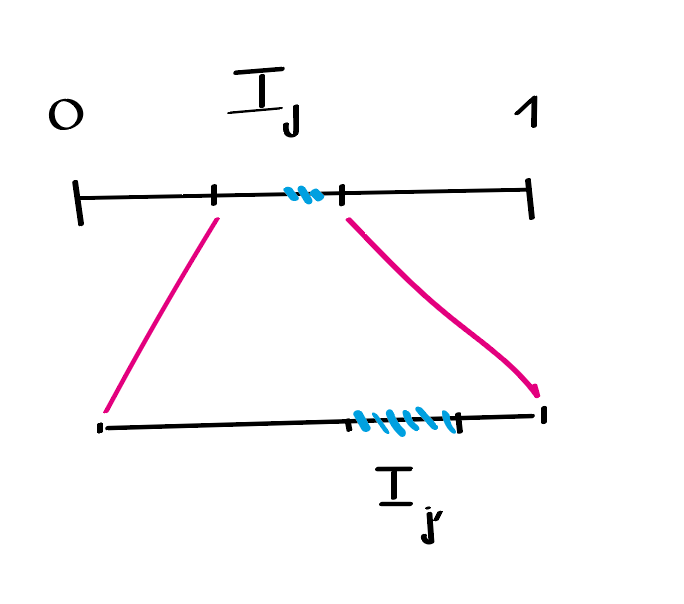
\includegraphics[scale = 0.3]{interval.png}
\end{figure}
%\pau
Or
$$
\mu_m^{\otimes \N}(C_{n, \mathbf{w}}) = \prod_{j=0}^p P(\{w_j\}) = \frac{1}{m^{p+1}}.
$$
\end{frame}

\begin{frame}
\textbf{8.} L'ensemble $\complement Z$ des points $m$-adiques est d\'enombrable, notons le $\{y_k,~�k\in\N\}$. On a alors
$$
\mathrm{Leb}\left(\complement Z\right) = \sum_{k} \mu(\{y_k\}) = 0.
$$
%\pau

\textbf{9.}
Si $\mathbf{x} \in H^{-1}(Z)$, alors $\mathbf{x}$ ne stationne pas \`a $1$ ni $m$ \`a partir d'un certain rang.

%\pau
\vspace{0.2cm}
On a
$$
\begin{aligned}
H(\sigma(\mathbf{x})) &= \sum_{k=1}^\infty \frac{x_{k+1} - 1}{m^k}�\mod \Z \\
%\pau
&= m H(\mathbf{x}) \mod \Z.
\end{aligned}
$$
%\pau
Il est clair que $x \in \R/\Z$ qui n'est pas $m$-adique admet exactement un ant\'ec\'edent par $H$, en regardant les nombres $x_k \in \{1, \dots, m\}$ ($k \in \N_{\geqslant 1}$) tels que
$$
x_k - 1 = \lfloor m^{k} x \rfloor \mod m,
$$
qui ne stationnent jamais \`a $1$ o\`u $m$.
\end{frame}

\end{document}





